% -----------------------------------------------------------------------------
% !Mode:: "TeX:Hard:UTF-8"
% PDFLaTeX this document and view or print it from Acrobat Reader!
% -----------------------------------------------------------------------------
% Preamble Starts here:
% -----------------------------------------------------------------------------
\documentclass{article}
\usepackage[colorlinks]{hyperref}
\usepackage{graphicx}
\usepackage[utf8]{inputenc} % UTF-8: PDFLaTeX
\usepackage[T1]{fontenc}
\usepackage[swedish]{babel}
%\usepackage{xltxtra} % UTF-8: XeLaTeX
% WinEdt's Bullets --------------------------------------------------------
% HINT: Use MiKTeX's Package Manager to install eurosym package!
% UTF-8 \u8:??? (€) Euro symbol is currently not supported with LaTeX
% unless the following package is used:
\usepackage{textcomp} % required for \texteuro
\usepackage{eurosym}  % required for \euro
% get a "nicer" looking euro symbol:
%\let\texteuro\euro   % if you want \texteuro=\euro
% WinEdt's Bullets --------------------------------------------------------
% Allow WinEdt's Bullets (placeholders) in TeX Files!
% The bullets (eg. in automatically generated tables)
% should be replaced by actual data. In WinEdt you can
% use Ctrl+Space (Tools menu -> Next Bullet) to navigate
% through bullets and replace them with "real" entries...
\catcode`\=13
\def{$\bowtie$}
% -----------------------------------------------------------------------------
% Document Starts here:
% -----------------------------------------------------------------------------

\begin{document}

\section{WinEdt and Unicode (UTF-8) encoding}

WinEdt is a unicode editor with support for UTF-8 or code page-specific
encoding. UTF-8 is the default format for TeX documents. This can be
configured through the Unicode section of the Options interface (or through
the Unicode page in Preferences dialog). Help explains the details.

If document's mode ends with submode :CPnum then the indicated code page is
used to load the file in unicode format. For example: TeX:CP1251 uses
Cyrillic code page.

A comment in the beginning of a TeX document:
\begin{verbatim}
    % !Mode:: "TeX:UTF-8"
\end{verbatim}
will ensure that a document is properly loaded and saved. A similar
convention is used by emacs:
\begin{verbatim}
    % -*-coding: utf-8 -*-
\end{verbatim}
WinEdt ``understands'' emacs coding directive for UTF-8.

Some unicode or UTF-8 documents start with a Byte Order Mark (BOM).
Unicode-aware applications can determine the coding of a document from its
BOM. Windows Notepad always includes BOM in unicode or UTF documents.
Unfortunately, the BOM signature also causes problems with many applications
and compilers (including TeX with UTF-8 encoding) and that makes it rather
useless...

Without BOM and without any convention as described above it is hard to
distinguish between UTF-8 and ANSI (code page-specific) documents.

Document Settings dialog has a page CP Converter. It can be used to change
document's format or reload the document in proper code page:

\medskip

\begin{center}
  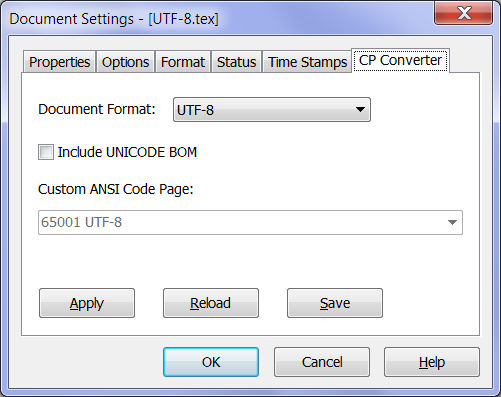
\includegraphics[width=3.0in]{Images/WinEdt-DocFormat}
\end{center}
Help in the dialog explains how to use this functionality.

% -----------------------------------------------------------------------------

\section{WinEdt and (Sub)Modes}

A document mode is initially determined from the filetype and is stored as a
local attribute of a file in WinEdt's File List (Project File). This works in
most cases for the main mode. However, bilingual users might want to tie
certain attributes (such as dictionaries) to submodes that may not be
apparent from the filetype.

\medskip

Instead of setting such modes in the Document Settings dialog or adopting a
practice to name your files with more than one filetype (eg. Paper.fr.tex) it
is possible to enter submodes (as comments) in the first (or second) line of
a document.

\bigskip

\noindent WinEdt modes can be specified as a comment:
\begin{verbatim}
    % !Mode:: "Mode:Submode:Submode"
\end{verbatim}

\noindent WinEdt also recognizes mode specification as used by emacs:
\begin{verbatim}
    % -*- mode: TeX -*-
    % -*- coding: utf-8 -*-
\end{verbatim}

\noindent It is also possible to specify mode and submode in a single
comment:
\begin{verbatim}
    % -*- TeX:DE:UTF-8 -*-
\end{verbatim}
Emacs might not recognize such specification and it is better to use WinEdt's
convention \verb|!Mode:: "TeX:DE:UTF-8"| as described above.

\noindent Furthermore, for TeX documents WinEdt also detects the language
submode from Babel and UTF-8 coding from the inputenc package:
\begin{verbatim}
    // Determine Language Submodes from babel:
    // \usepackage[french,german,italian,spanish]{babel}

    // Determine Coding (UTF-8) from the preamble:
    // \usepackage[utf8]{inputenc}
\end{verbatim}

This functionality is implemented thought the event handler macros that are
executed before a document is loaded into WinEdt. Event handlers are defined
in the Advanced section of the Options interface.

This ensures that WinEdt opens and treats the document properly. WinEdt's
Help explains how to use modes and submodes...

\noindent The actual macro that is by default called from this event handler
is
\begin{verbatim}
    %b\Macros\Events\GetMode.edt
\end{verbatim}

If for some reason mode detection (or some portion of it) from comments is
unwanted for your style of work you can edit this macro and comment out
unwanted portions or make any other desirable changes. However, note that
this macro is executed frequently and it has to be fast or else you'll notice
delays when opening documents or even when collecting data in previously
un-opened documents...

% -----------------------------------------------------------------------------

\section{TeX and International Characters (UTF-8)}

Putting
\begin{verbatim}
  \usepackage[utf8]{inputenc}
\end{verbatim}
enables you to use UTF-8 (unicode) coding in LaTeX documents. As long as you
open the document in WinEdt in UTF-8 mode you see the same characters in
WinEdt as in your compiled document (as is the case with this UTF-8
document):

\bigskip

 \noindent \texttt{À Á Â Ã Ä Å Æ Ç È É Ê Ë Ì Í Î Ï Ñ Ò Ó Ô Õ Ö Ø Œ Ù Ú Û Ü Ý Ÿ Š ß ¡}

 \noindent \texttt{à á â ã ä å æ ç è é ê ë ì í î ï ñ ò ó ô õ ö ø œ ù ú û ü ý ÿ š € ¿}

 \noindent \texttt{† ‡ § ¶ © ® Č Š Ž č š ž}

\bigskip

 \noindent {À Á Â Ã Ä Å Æ Ç È É Ê Ë Ì Í Î Ï Ñ Ò Ó Ô Õ Ö Ø Œ Ù Ú Û Ü Ý Ÿ Š ß ¡}

 \noindent {à á â ã ä å æ ç è é ê ë ì í î ï ñ ò ó ô õ ö ø œ ù ú û ü ý ÿ š € ¿}

 \noindent {† ‡ § ¶ © ® Č Š Ž č š ž}

\bigskip

Not all UTF-8 characters are currently supported by LaTeX unless you load
extra packages. For example the \euro\ (€) symbol requires:

\begin{verbatim}
  \usepackage{textcomp} % required for \texteuro
  \usepackage{eurosym}  % required for \euro
  % get a "nicer" looking euro symbol:
  %\let\texteuro\euro   % if you want \texteuro=\euro
\end{verbatim}

Note the difference between the shape of the \verb"\euro" (\euro) and
\verb"\texteuro" (\texteuro) symbols. Such issues are non-WinEdt related and
you will have to consult TeX's documentation or, if needed, seek help on the
appropriate forum (such as TeX Newsgroup where \LaTeX\ related topics are
discussed).

\bigskip

\noindent Our preamble contains:

\begin{verbatim}
  \catcode`\=13
  \def{$\bowtie$}
\end{verbatim}

\noindent This allows \TeX\ to process an ``empty'' tabular environment from
WinEdt's Insert menu. Bullets are represented by :

\begin{center}
  \begin{tabular}{|c|c|c|c|c|}
    \hline
    % after \\: \hline or \cline{col1-col2} \cline{col3-col4} ...
     &  &  &  &  \\
    \hline
     &  &  &  &  \\
     &  &  &  &  \\
     &  &  &  &  \\
    \hline
  \end{tabular}
\end{center}

\noindent \emph{In WinEdt you can use Ctrl+Space (Tools menu -> Next Bullet)
to move through placeholders and fill-in the actual data.}

\newpage

% -----------------------------------------------------------------------------

\section{Translation Tables}

If you prefer your documents to contain plain \TeX\ notation for
international characters (eg. \verb"\`{A}" stands for \texttt{À}) then you
should consider applying WinEdt's read and write translation tables. This
will make working with WinEdt more comfortable and it is required if you want
to take advantage of WinEdt's spell checking ability with international
dictionaries.

\medskip

\emph{WinEdt can convert certain strings into their unicode equivalents when
the file is being read and then translate these characters back to the
original strings representing international characters in \TeX\ notation.}

\medskip

Suitable translation tables for TeX mode are already defined (but not
enabled) in the default settings: see Options interface. The help in this
interface provides the details.

\bigskip

For example, the default \verb"TeX_Read" and \verb"TeX_Write" translation
table contain definitions like:

\begin{verbatim}
          "{\ss}" -> "ß"               "ß" -> "{\ss}"
          "{\AA}" -> "Å"               "Å" -> "{\AA}"
          "{\AE}" -> "Æ"               "Æ" -> "{\AE}"
          "{\aa}" -> "å"               "å" -> "{\aa}"
          "{\ae}" -> "æ"               "æ" -> "{\ae}"
          "{\OE}" -> "Œ"               "Œ" -> "{\OE}"
          "{\oe}" -> "œ"               "œ" -> "{\oe}"
          "{\O}" -> "Ø"                "Ø" -> "{\O}"
          "{\o}" -> "ø"                "ø" -> "{\o}"
          "\c{C}" -> "Ç"               "Ç" -> "\c{C}"
          "\c{c}" -> "ç"               "ç" -> "\c{c}"
          "\^{A}" -> "Â"               "Â" -> "\^{A}"
          "\~{A}" -> "Ã"               "Ã" -> "\~{A}"
          "\""{A}" -> "Ä"              "Ä" -> "\""{A}"

          etc...

\end{verbatim}

\emph{Note that the last item is not a ``typo''! To specify double quotes
inside a double-quoted string they have to be repeated twice! Failing to
observe this convention may completely corrupt WinEdt's translation table.}

\bigskip

The read translation table supports two notations (eg. \verb"\^{A}" and
\verb"{\^A}"). The write translation table \verb"TeX_Write" is the inverse of
the read translation table (except that it uses the first, preferable,
notation where applicable). You should use translation tables with some care:
make a backup copy of your documents until you verify that the tables are set
up correctly. Careless application of translation tables may irreversibly
corrupt your documents (just like a global replace)!!!

\end{document}

% -----------------------------------------------------------------------------
